\subsubsection{Caso d'uso UC8.1.4: Creazione domanda vero/falso}
	\label{UC8.1.4}
	\begin{figure}[h]
		\centering
			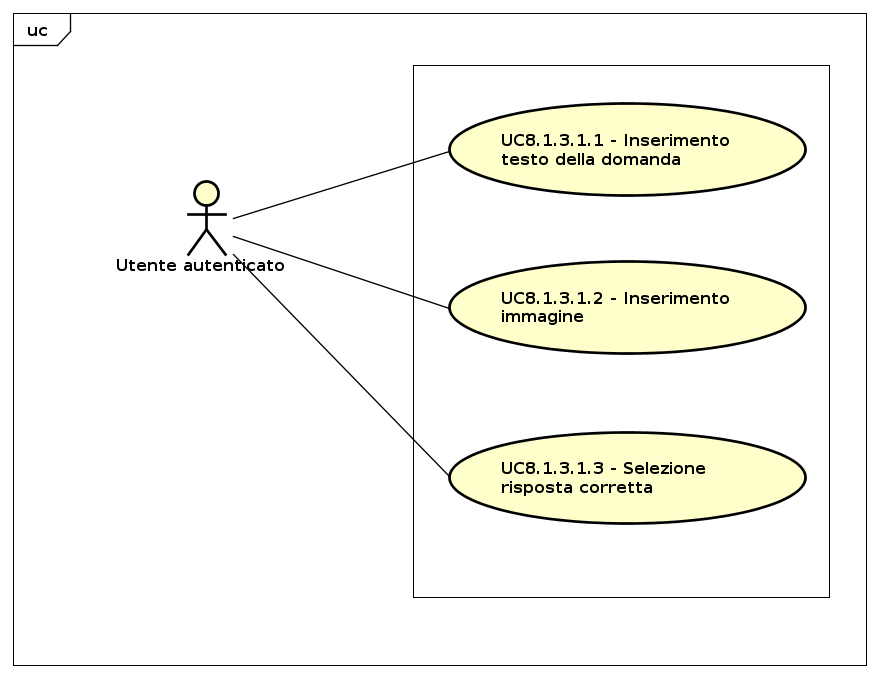
\includegraphics[scale=0.45,keepaspectratio]{UML/UC8_1_4.png}
		\caption{UC8.1.4: Creazione domanda vero/falso}
	\end{figure}
	\FloatBarrier
	\begin{itemize}
		\item
			\textbf{Attori}: utente autenticato, utente autenticato pro;
		\item		
			\textbf{Descrizione}: l'attore può utilizzare la procedura guidata per la creazione di una domanda vero/falso;
		\item
			\textbf{Precondizione}: il sistema presenta all'attore la procedura guidata per la creazione di una domanda vero/falso; 
		\item
			\textbf{Postcondizione}: l'attore ha creato una domanda vero/falso;
		\item
			\textbf{Scenario principale}:
	       		\begin{enumerate}
	       			\item
	       			L'attore può inserire il testo della domanda (UC8.1.4.1);
	       			\item
	       			L'attore può inserire un'immagine relativa al testo della domanda (UC8.1.4.2);
					\item
					L'attore può indicare la risposta corretta tramite uno strumento di selezione (UC8.1.4.3).
	 			\end{enumerate}
	\end{itemize}

\subsubsection{Caso d'uso UC8.1.4.1: Inserimento testo della domanda}
	\begin{itemize}
		\item
			\textbf{Attori}: utente autenticato, utente autenticato pro;
		\item		
			\textbf{Descrizione}: l'attore può inserire il testo della domanda;
		\item
			\textbf{Precondizione}: il sistema presenta all'attore lo spazio destinato all'inserimento del testo della domanda; 
		\item
			\textbf{Postcondizione}: l'attore ha inserito il testo della domanda;
		\item
			\textbf{Scenario principale}: l'attore inserisce il testo della domanda. 
	 			
	\end{itemize}
	
\subsubsection{Caso d'uso UC8.1.4.2: Inserimento immagine}
	\begin{itemize}
		\item
			\textbf{Attori}: utente autenticato, utente autenticato pro;
		\item		
			\textbf{Descrizione}: l'attore può inserire un'immagine relativa al testo della domanda;
		\item
			\textbf{Precondizione}: il sistema presenta all'attore la funzionalità di inserimento di un immagine; 
		\item
			\textbf{Postcondizione}: l'attore ha inserito un'immagine relativa al testo della domanda;
		\item
			\textbf{Scenario principale}: l'attore inserisce un'immagine.						
	\end{itemize}
	

\subsubsection{Caso d'uso UC8.1.4.3: Selezione risposta corretta}
	\begin{itemize}
		\item
			\textbf{Attori}: utente autenticato, utente autenticato pro;
		\item		
			\textbf{Descrizione}: l'attore può indicare la risposta corretta;
		\item
			\textbf{Precondizione}: il sistema presenta all'attore la funzionalità di selezione di una risposta corretta; 
		\item
			\textbf{Postcondizione}: l'attore ha selezionato la risposta corretta;
		\item
			\textbf{Scenario principale}: l'attore indica la risposta corretta.  			
	\end{itemize}